
%(BEGIN_QUESTION)
% Copyright 2011, Tony R. Kuphaldt, released under the Creative Commons Attribution License (v 1.0)
% This means you may do almost anything with this work of mine, so long as you give me proper credit

This water filter's discharge pressure is controlled by a PID controller, throttling the amount of water returned to the sump:

$$\includegraphics[width=15.5cm]{i00434x01.eps}$$

An operator tells you there is a problem with this system, though: the controller faceplate registers 146 PSI of water pressure, with a setpoint at 100 PSI.  You happen to notice that the bargraph on the controller faceplate showing output is at 100\%.  Another operator in the field (near the exchanger) reports via radio that the control valve stem is at the ``closed'' position, and that the pressure gauge mounted on the filter's discharge line registers 143 PSI.

\vskip 10pt

Another instrument technician happens to be with you, and recommends you connect a multimeter to the transmitter's signal wiring to measure the 4-20 mA signal.  Explain why this test would be a waste of time, and propose a better test for helping to pinpoint the location of the fault.

\vskip 20pt \vbox{\hrule \hbox{\strut \vrule{} {\bf Suggestions for Socratic discussion} \vrule} \hrule}

\begin{itemize}
\item{} A valuable principle to apply in a diagnostic scenario such as this is {\it correspondence}: identifying which field variables correspond with their respective controller faceplate displays, and which do not.  Apply this comparative test to the scenario described, and use it to explain why the technician's proposed test was probably not the best first step.
\item{} Determine the proper action for this loop controller (direct or reverse).
\item{} For those who have studied PID tuning, qualitatively determine appropriate P, I, and D parameters for the loop controller based on how you would expect this process to respond.
\end{itemize}

\underbar{file i00434}
%(END_QUESTION)





%(BEGIN_ANSWER)

The reason that the technician's proposed test would have been a waste of time is because the controller is already registering a reasonable pressure (approximately the same as the field-mounted gauge).  In other words, the controller PV indication corresponds with the gauge, suggesting there is no problem in that (input) portion of the control system.
 
%(END_ANSWER)





%(BEGIN_NOTES)

The controller's ``decision'' to open the return valve wide makes sense from the perspective of PV $>$ SP, so the real question here is ``why isn't the valve responding to the controller's output?''  The output indication does not correspond with the valve stem position, suggesting a problem on the FCE (output) side of the control system.  Possibilities include:

\begin{itemize}
\item{} Loss of instrument air to I/P
\item{} Wiring failed open or shorted between controller and I/P
\item{} Large air leak in valve diaphragm
\end{itemize}

A good ``next step'' would be to inspect the valve's stem position, to see if it is actually wide-open as the controller is commanding it to be.

%INDEX% Basics, control loop troubleshooting: isolating area of fault by correspondence

%(END_NOTES)


